\documentclass [aspectratio=169]{beamer}
\beamertemplatenavigationsymbolsempty
\usetheme{Boadilla}
\usepackage{textpos} % package for the positioning
\usepackage[]{graphicx}
\usepackage{graphicx}
\usepackage{float}
\usepackage{hyperref}
\usepackage{caption}
\usepackage{subcaption}
\usepackage{algorithm,algpseudocode}
\usepackage[export]{adjustbox}
\usepackage{tikz}
\usetikzlibrary{positioning}

\usepackage[square,numbers]{natbib}
\usepackage[byname]{smartref}
\usetikzlibrary{positioning}
\usetikzlibrary{arrows, shapes, decorations, automata, backgrounds, fit, petri, calc}

\newcommand*{\logofont}{\fontfamily{phv}\selectfont}

\definecolor{uwopurple}{RGB}{79,38,131} % official purple color for uwo

\title[]{\vspace{60pt} \\
SleepGCN-Transformer: A Hybrid Graph Convolutional and Transformer Network for Sleep Stage Classification} % Change the lecture topic right here!
%\subtitle{n}
\author[]{Tanmay Rathod }
\large \institute[]{Under the guidance: Dr. Santosh Kumar Satapathy\\ [5pt]
Assistant Professor, Department of ICT, PDPU Gandhinagar}

\date{February 19, 2025}

% Math notations
\newtheorem{thm}{Theorem}[section]
\newtheorem{lem}[thm]{Lemma}

\newtheorem{defn}[thm]{Definition}
\newtheorem{eg}[thm]{Example}
\newtheorem{ex}[thm]{Exercise}
\newtheorem{conj}[thm]{Conjecture}
\newtheorem{cor}[thm]{Corollary}
\newtheorem{claim}[thm]{Claim}
\newtheorem{rmk}[thm]{Remark}

\newcommand{\ie}{\emph{i.e.} }
\newcommand{\cf}{\emph{cf.} }
\newcommand{\into}{\hookrightarrow}
\newcommand{\dirac}{\slashed{\partial}}
\newcommand{\R}{\mathbb{R}}
\newcommand{\C}{\mathbb{C}}
\newcommand{\Z}{\mathbb{Z}}
\newcommand{\N}{\mathbb{N}}
\newcommand{\Q}{\mathbb{Q}}
\newcommand{\LieT}{\mathfrak{t}}
\newcommand{\T}{\mathbb{T}}
\newcommand{\A}{\mathds{A}}
\newcommand{\E}{\mathbb{E}}
\newcommand{\Prob}{\mathbb{P}}
\newcommand{\Var}{\text{Var}}
\newcommand\equalhat{%
\let\savearraystretch\arraystretch
\renewcommand\arraystretch{0.3}
\begin{array}{c}
\stretchto{
    \scalerel*[\widthof{=}]{\wedge}
    {\rule{1ex}{3ex}}%
}{0.5ex}\\ 
=%
\end{array}
\let\arraystretch\savearraystretch
}

% set color
\setbeamercolor{title in head/foot}{bg=white}
\setbeamercolor{author in head/foot}{bg=white}
\setbeamercolor{date in head/foot}{fg=uwopurple}
\setbeamercolor{date in head/foot}{bg=white}
\setbeamercolor{title}{fg=uwopurple}
\setbeamerfont{title}{series=\bfseries}
\setbeamercolor{frametitle}{fg=uwopurple}
\setbeamerfont{frametitle}{series=\bfseries}
\setbeamercolor{block title}{bg=uwopurple!30,fg=black}
\setbeamercolor{item}{fg=uwopurple}
\setbeamercolor{caption name}{fg=uwopurple!70!}









 

 
\begin{document}

{
\setbeamertemplate{logo}{}
\begin{frame}
    \titlepage
    \begin{textblock*}{4cm}(0.5cm,-7.3cm)
        
\includegraphics[width=4cm]{figures/pdpu logo-.png}
    \end{textblock*}
    \begin{textblock*}{8cm}(5.0cm,-7.0cm)
        \huge \color{uwopurple}{$\Bigr\rvert$ \hspace{0.15cm} \textbf{Project Seminar}} % Change the lecture # right here! 
    \end{textblock*}
\end{frame}
}




\begin{frame}{Table of Contents}

    \begin{block}{}
        \begin{itemize}
            \item \textbf{1. Abstract}
            \item \textbf{2. Introduction}
            \item \textbf{3. Problem Statement}
            \item \textbf{4. Methodology}
            \item \textbf{5. Results}
            \item \textbf{6. Future Plan \& Conclusion}
        \end{itemize}
    \end{block}
\end{frame}


     \begin{frame}{Abstract}
    \textbf{Dataset:} \textbf{SleepEDF} dataset. \\[5pt]

    \textbf{Preprocessing:} Using 4 selected channels:  
    \begin{itemize}
        \item EEG Fpz-Cz
        \item EEG Pz-Oz
        \item EMG submental
        \item EOG horizontal
    \end{itemize}

    \textbf{Methodology:}  
    \begin{itemize}
        \item \textbf{Graph Convolutional Neural Network (GCN)} 
        \item \textbf{Transformer Encoder}  
    \end{itemize}

    \textbf{Results:}  
    \begin{itemize}
        \item \textbf{Epoch 20/20:} Train Loss: \textbf{0.1413}, Train Acc: \textbf{93.12\%}  
        \item Validation Loss: \textbf{0.1390}, Validation Accuracy: \textbf{93.04\%}  
    \end{itemize}
\end{frame}
   
 
     \begin{frame}{Introduction}
	\begin{columns}
		% Left Column: EEG Channels and Sleep Stages Table (Now on the Left Side)
		\column{0.50\textwidth}
		\textbf{SleepEDF Channels:}
		\begin{itemize}
			\item EEG Fpz-Cz
			\item EEG Pz-Oz
			\item EMG submental
			\item EOG horizontal
		\end{itemize}
		
		\vspace{10pt}
		
		\textbf{Sleep Stages and Frequency Ranges:}
		\begin{table}
			\centering
			\renewcommand{\arraystretch}{1.2}
			\begin{tabular}{|c|c|}
				\hline
				\textbf{Sleep Stage} & \textbf{Frequency (Hz)} \\
				\hline
				Wake (Beta) & 12-30 \\
				N1 (Light Sleep) & 4-8 \\
				N2 (Moderate Sleep) & 4-6 \\
				N3 (Deep Sleep) & 0.5-4 \\
				REM (Theta) & 4-6 \\
				\hline
			\end{tabular}
		\end{table}
		
		% Right Column: Figure (Now on the Right Side)
		\column{0.50\textwidth}
		\begin{figure}
			\centering
			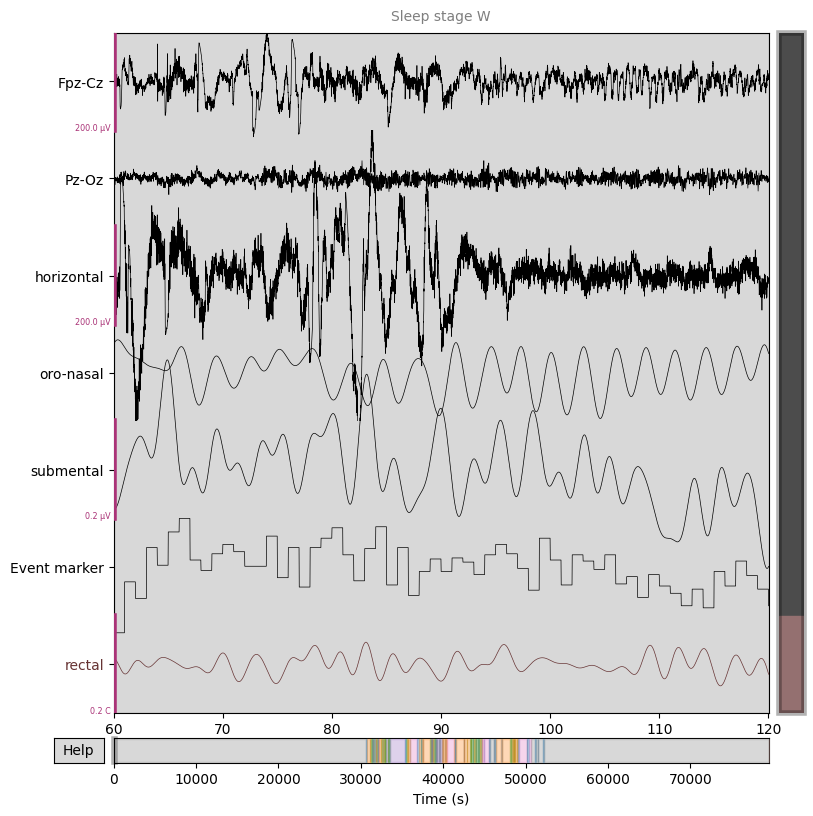
\includegraphics[width=\linewidth]{Sleep EDF Data Visulization.png} % Replace with your actual figure
			\caption{Sleep Stage Representation}
		\end{figure}
	\end{columns}
\end{frame}
   
    \begin{frame}{Problem Statement}
    \begin{block}{\centering \textbf{Problem Statement}}
        \centering
        \textbf{Using  SleepGCN-Transformer: A Hybrid Graph Convolutional and Transformer Network for Sleep Stage Classification}
    \end{block}
\end{frame}


 \begin{frame}{Methodology}
    \centering
    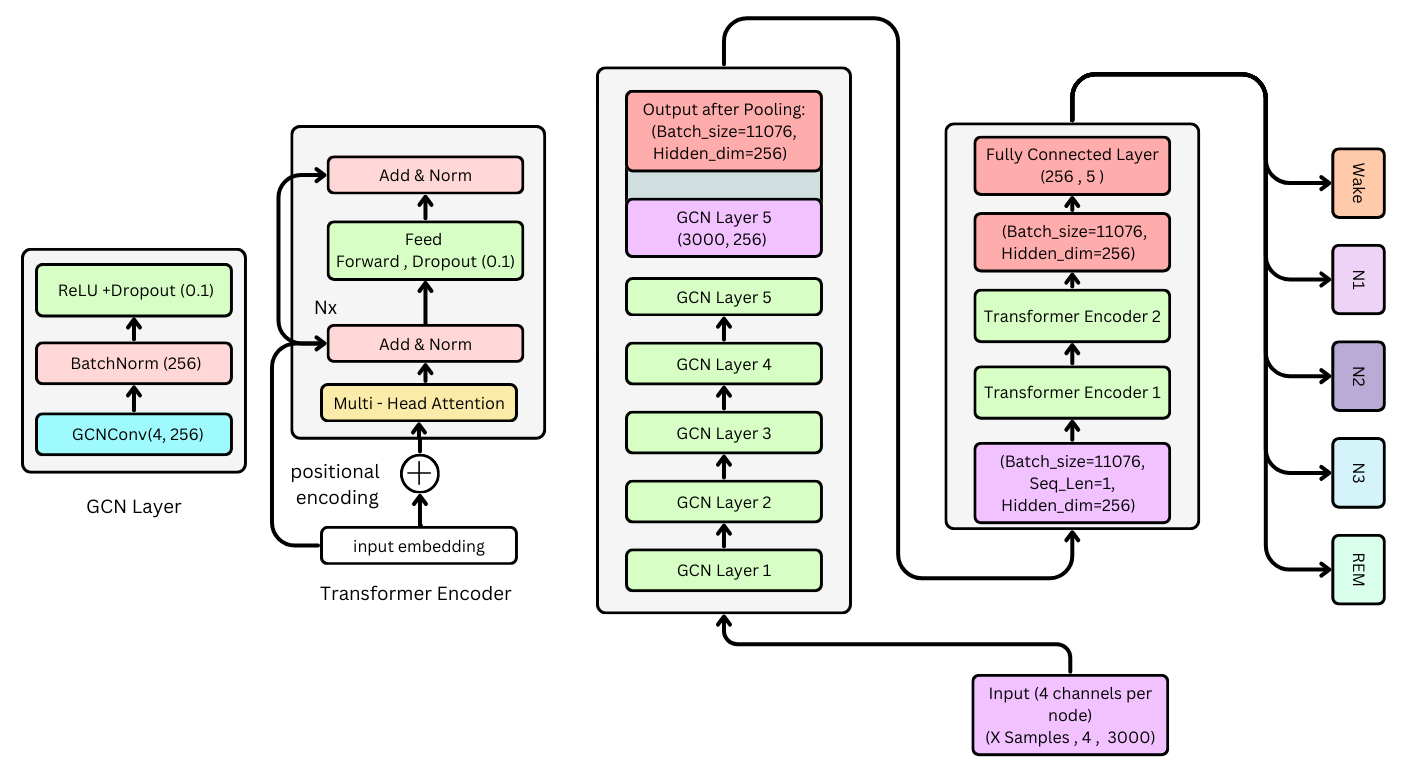
\includegraphics[width=0.85\linewidth]{figures/Architechture.png} % Slightly smaller image

        \small \textbf{Figure:} Proposed SleepGCN-Transformer Architecture % Smaller caption
\end{frame}

\begin{frame}{Methodology: Preprocessing}
    \begin{columns}
        % Left Column: Channel Selection
        \column{0.50\textwidth}
        \textbf{Channel Selection:}
        \begin{itemize}
            \item Extracting four relevant EEG channels:
            \begin{itemize}
                \item EEG Fpz-Cz
                \item EEG Pz-Oz
                \item EMG submental
                \item EOG horizontal
            \end{itemize}
        \end{itemize}

        % Right Column: Sleep Stage Mapping
        \column{0.50\textwidth}
        \textbf{Sleep Stage Mapping:}
        \begin{table}[]
            \centering
            \renewcommand{\arraystretch}{1.2}
            \begin{tabular}{|c|c|}
                \hline
                \textbf{Original Stage} & \textbf{Mapped Label} \\
                \hline
                Sleep stage W  & 0 \\
                Sleep stage 1  & 1 \\
                Sleep stage 2  & 2 \\
                Sleep stage 3  & 3 \\
                Sleep stage 4  & 3 \\
                Sleep stage R  & 4 \\
                \hline
            \end{tabular}
        \end{table}
    \end{columns}
\end{frame}









\begin{frame}{Methodology: Preprocessing}
    \textbf{Epoch Segmentation:}
    \begin{itemize}
        \item EEG signals are segmented into 30-second epochs.
        \item Each epoch contains 3000 samples per channel.
    \end{itemize}

    \vspace{10pt}
    \textbf{Band-Pass Filtering:}
    \begin{itemize}
        \item A band-pass filter (0.3 - 30 Hz) is applied.
        \item Signals above 30 Hz are removed to eliminate noise.
    \end{itemize}

    \vspace{10pt}
    \textbf{Final Data Shape:}  
    \[
    \text{[X, 4, 3000]}  
    \]

    \end{frame}


\begin{frame}{Methodology: Graph Dataset Creation}

    \begin{columns}
    
        % Left Column: Graph Adjacency Matrix
        \column{0.50\textwidth}
        \textbf{Graph Adjacency Matrix (Edge Weights):}
        \centering
        \renewcommand{\arraystretch}{1.2}
        \resizebox{\linewidth}{!}{ % Ensures table fits within the column
            \begin{tabular}{|c|c|c|c|c|}
                \hline
                & \textbf{Fpz-Cz} & \textbf{Pz-Oz} & \textbf{EMG} & \textbf{EOG} \\
                \hline
                \textbf{Fpz-Cz} & 0   & 0.9 & 0.6 & 0.6 \\
                \textbf{Pz-Oz}  & 0.9 & 0   & 0.6 & 0.6 \\
                \textbf{EMG}    & 0.6 & 0.6 & 0   & 0.5 \\
                \textbf{EOG}    & 0.6 & 0.6 & 0.5 & 0   \\
                \hline
            \end{tabular}
        }

        \vspace{8pt}

        \textbf{Dataset Information:}
        \begin{itemize}
            \item Total Samples: 11,076
            \item Example Sample Format:
        \end{itemize}

  
        \text{Data(x=[3000, 4], edge\_index=[2, 12],}
  
        \text{edge\_attr=[12], y=[1])}
      

        % Right Column: Graph Representation
        \column{0.50\textwidth}
        \centering
        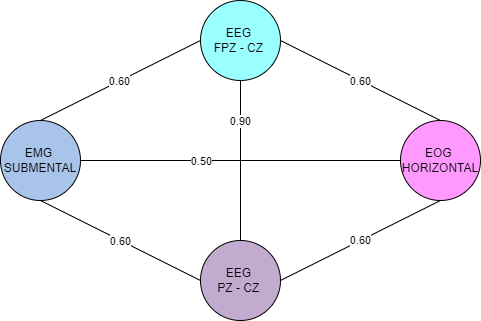
\includegraphics[width=0.85\linewidth]{figures/Graph Weightage.png} % Replace with actual graph image

        {\textcolor{purple}{\small Graph Representation of EEG Channels}}

    \end{columns}
\end{frame}



\begin{frame}{Methodology: Graph Convolutional Layer}
    \begin{columns}[c] % Align columns at the center for better layout

        % Left Column: Explanation and Data Shapes
        \column{0.50\textwidth}
        
        \textbf{Graph Convolutional Layer (GCL)}
        \vspace{5pt}
        \begin{itemize}
            \item Captures spatial relationships in EEG signals.
            \item Learns connectivity patterns between EEG channels.
            \item Enhances feature extraction by leveraging graph structures.
        \end{itemize}

        \vspace{8pt} % Adjust spacing for better layout
        \textbf{Tensor Shapes for GCL Input:}
        \vspace{3pt}
        \begin{itemize}
            \item \textbf{X\_all}: (11076, 4, 3000)
            \item \textbf{Y\_all}: (11076,)
            \item \textbf{X\_tensor}: \texttt{torch.Size([11076, 4, 3000])}
            \item \textbf{Y\_tensor}: \texttt{torch.Size([11076])}
            \item \textbf{Sample x}: \texttt{torch.Size([3000, 4])}
            \item \textbf{Sample edge\_index}: \texttt{torch.Size([2, 12])}
            \item \textbf{Sample y}: \texttt{torch.Size([1])}
        \end{itemize}

        % Right Column: GCL Image with Proper Caption
        \column{0.50\textwidth}
        \centering
        \vspace{-10pt} % Adjust vertical spacing for better fit
        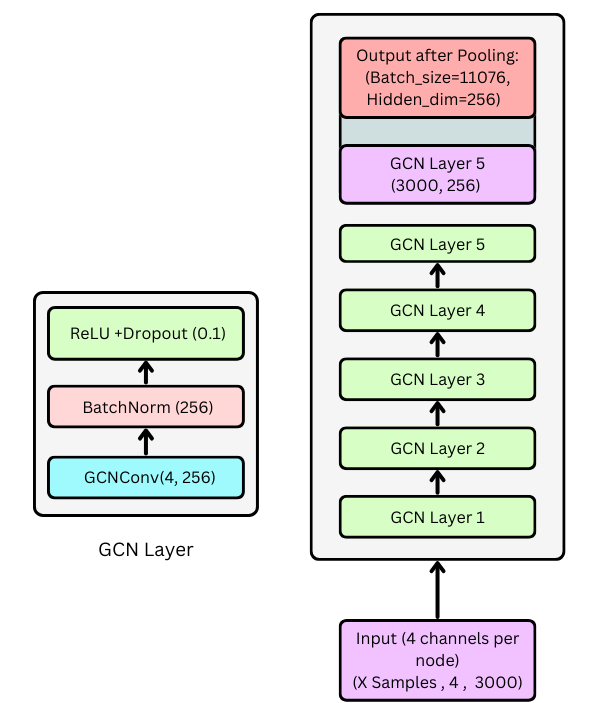
\includegraphics[width=0.6\linewidth]{figures/Graph Convolution Neural Network.png} % Adjusted path and width

        % Proper caption placement
        \vspace{0.3cm}
        \small{\textcolor{uwopurple}{Graph Convolutional Layer Representation}}

    \end{columns}
\end{frame}


\begin{frame}{Methodology: GCN Tensor Details and Global Pooling}
    \centering % Center the entire content for better alignment

    \textbf{Additional Tensor Shapes for GCL:}
    \vspace{5pt} % Adjust spacing for better readability
    \begin{itemize}
        \item \textbf{Sample x}: \texttt{torch.Size([3000, 4])}
        \item \textbf{Sample edge\_index}: \texttt{torch.Size([2, 12])}
        \item \textbf{Sample y}: \texttt{torch.Size([1])}
    \end{itemize}

    \vspace{10pt} % Space between sections
    \textbf{Global Mean Pooling:}
    \vspace{5pt}
    \begin{itemize}
        \item \textbf{Input:} Node embeddings from GCN layers (e.g., (3000, 256))
        \item \textbf{Operation:} Mean pooling over nodes based on batch indices
        \item \textbf{Output:} Graph-level embedding (e.g., (Batch\_size=11076, 256))
    \end{itemize}

\end{frame}



\begin{frame}{Methodology: Transformer Encoder}
    \begin{columns}

        % Left Column: Details
        \column{0.50\textwidth}

        \textbf{\large Transformer Encoder Overview}
        \vspace{5pt}
        \begin{itemize}
            \item \textbf{Preprocessing:} Expand graph embedding to \texttt{(Batch, 1, 256)}
            \item \textbf{Transformer Encoder:} 
            \begin{itemize}
                \item \textbf{2 Transformer Encoder Layers} with:
                \begin{itemize}
                    \item \textbf{d\_model = 256}
                    \item \textbf{nhead = 4}
                    \item \textbf{dropout = 0.1}
                    \item \texttt{batch\_first=True}
                \end{itemize}
            \end{itemize}
            \item \textbf{Postprocessing:} Squeeze output to \texttt{(Batch, 256)}
        \end{itemize}

        \vspace{10pt}
        \textbf{\large Fully Connected Layer}
        \vspace{5pt}
        \begin{itemize}
            \item \textbf{Linear Layer:} \texttt{Linear(256 → 5)}
            \item \textbf{Output:} Logits for 5-class classification
        \end{itemize}

        % Right Column: Transformer Figure
        \column{0.50\textwidth}
        \centering
        % \vspace{-}
        \includegraphics[width=\linewidth]{figures/Transformer.png} % Replace with actual image
        \vspace{2pt}
        \captionof{figure}{\textcolor{uwopurple}{Transformer Encoder Architecture}}

    \end{columns}
\end{frame}

\begin{frame}{Methodology: Why Focal Loss Instead of Standard Cross-Entropy?}

    \textbf{\large Motivation for Focal Loss}
    \vspace{5pt}
    \begin{itemize}
        \item Standard Cross-Entropy treats all samples equally, leading to bias towards majority classes.
        \item In imbalanced datasets, minority class predictions get suppressed.
        \item \textbf{Focal Loss} dynamically adjusts loss contribution based on prediction confidence.
        \item It reduces the importance of well-classified samples and focuses more on hard-to-classify ones.
    \end{itemize}

    \vspace{10pt}
    \textbf{\large Key Features of Focal Loss}
    \vspace{5pt}
    \begin{itemize}
        \item Introduces a focusing parameter \( \gamma \) to adjust class weighting.
        \item Includes class weighting factor \( \alpha \) to handle imbalance.
        \item Works well for highly imbalanced datasets in classification tasks.
    \end{itemize}

\end{frame}
\begin{frame}{Methodology: Focal Loss Formulation}

    \textbf{\large Mathematical Formulation}
    \vspace{5pt}

    \[
    \text{FL}(p_t) = -\alpha (1 - p_t)^{\gamma} \log(p_t)
    \]

    where:
    \begin{itemize}
        \item \( p_t \) is the predicted probability for the target class.
        \item \( \alpha \) is the weighting factor for class imbalance.
        \item \( \gamma \) is the focusing parameter (higher values focus more on hard examples).
    \end{itemize}

    \vspace{10pt}
    \textbf{\large Implementation Details}
    \vspace{5pt}
    \begin{itemize}
        \item Label smoothing:  
              \[
              y_{\text{smooth}} = y(1 - \epsilon) + \frac{\epsilon}{C}
              \]
        \item Prevents log(0) issue by adding a small constant \( \epsilon \).
        \item PyTorch-based computation:  
              \[
              \mathcal{L} = \alpha (1 - p)^{\gamma} (-y_{\text{smooth}} \log p)
              \]
    \end{itemize}

\end{frame}


\begin{frame}{Why Use a Learning Rate Scheduler?}

    \textbf{\large Importance of Learning Rate Scheduling}
    \vspace{5pt}
    \begin{itemize}
        \item The learning rate is crucial for training deep models efficiently.
        \item A high learning rate can lead to divergence, while a low one may cause slow convergence.
        \item Adaptive learning rate schedules help balance stability and speed.
    \end{itemize}

    \vspace{10pt}
    \textbf{\large Why CosineAnnealingLR?}
    \vspace{5pt}
    \begin{itemize}
        \item Smoothly reduces the learning rate following a cosine decay.
        \item Starts with a large step size for exploration and gradually fine-tunes.
        \item Helps avoid sharp drops in the learning rate, improving generalization.
    \end{itemize}

\end{frame}



\begin{frame}{Cosine Annealing Learning Rate Decay}

    \textbf{\large Cosine Annealing Formula:}
    \[
    \eta_t = \eta_{\text{min}} + \frac{1}{2} (\eta_{\text{max}} - \eta_{\text{min}}) 
    \left( 1 + \cos \left( \frac{T_{cur}}{T_{max}} \pi \right) \right)
    \]
    where:
    \begin{itemize}
        \item \( \eta_t \) is the learning rate at epoch \( t \).
        \item \( \eta_{\text{max}} \) and \( \eta_{\text{min}} \) are the max/min learning rates.
        \item \( T_{cur} \) is the current epoch.
        \item \( T_{max} \) is the total number of epochs.
    \end{itemize}

    \vspace{10pt}
    \textbf{\large Key Benefits:}
    \begin{itemize}
        \item Encourages large updates early in training.
        \item Smoothly transitions into finer updates as training progresses.
        \item Helps the model avoid getting stuck in poor local minima.
    \end{itemize}

\end{frame}


\begin{frame}{Training Methodology: Overview}

    \textbf{\large SleepTrainer Class: Key Features}
    \vspace{5pt}
    \begin{itemize}
        \item Handles model training, validation, and optimization.
        \item Uses \textbf{Focal Loss} to address class imbalance.
        \item Applies \textbf{CosineAnnealingLR} scheduler for smooth learning rate decay.
    \end{itemize}

    \vspace{10pt}
    \textbf{\large Training Process}
    \vspace{5pt}
    \begin{enumerate}
        \item Compute class weights for imbalanced data.
        \item Iterate through training batches, compute loss and update weights.
        \item Validate model performance on a separate validation set.
        \item Adjust learning rate dynamically using a scheduler.
    \end{enumerate}

\end{frame}


\begin{frame}{Training Methodology: Hyperparameters}

    \textbf{\large Key Hyperparameters}
    \vspace{5pt}
    \begin{itemize}
        \item \textbf{Batch Size:} 32  \hfill 
        \item \textbf{Learning Rate:} 0.0003  \hfill
        \item \textbf{Weight Decay:} \( 1e^{-4} \)  \hfill 
        \item \textbf{Epochs:} 20  \hfill 
        \item \textbf{Optimizer:} AdamW  \hfill 
    \end{itemize}

    \vspace{10pt}
    \textbf{\large Learning Rate Scheduler: CosineAnnealingLR}
    \begin{itemize}
        \item Gradually reduces learning rate over time for smooth convergence.
        \item Helps prevent sudden drops in performance.
    \end{itemize}

\end{frame}

\begin{frame}{Training Methodology: Handling Class Imbalance}

    \textbf{\large Why Compute Class Weights?}
    \vspace{5pt}
    \begin{itemize}
        \item EEG sleep data is imbalanced, with some sleep stages appearing more frequently.
        \item Without weighting, the model may favor majority classes.
        \item Weights ensure rare classes contribute more to the loss.
    \end{itemize}

    \vspace{10pt}
    \textbf{\large Class Weight Computation}
    \vspace{5pt}
    \[
    w_c = \left( \frac{\text{Total Samples}}{\text{Class Count} + 1} \right)^{0.5}
    \]
    where:
    \begin{itemize}
        \item \( w_c \) is the computed weight for class \( c \).
        \item Small classes receive higher weights.
        \item Weights are applied to Focal Loss for training.
    \end{itemize}

\end{frame}




 
\begin{frame}{Testing Data Distribution Analysis}

    \begin{columns}

        % Left Column: Explanation
        \column{0.50\textwidth}
        \textbf{Why Ensure Balanced Testing Data?}
        \begin{itemize}
     \item Prevents bias toward majority classes.
        \item Ensures the model's performance is fairly evaluated.
        \item Helps achieve reliable generalization across all sleep stages.
           \item The figure shows the normalized class distribution during testing.
        \item Each class maintains an equalized density, avoiding class imbalance.
        \item This confirms that the model's evaluation is not biased toward any specific sleep stage.
        \end{itemize}

        % Right Column: Sampling Density Plot
        \column{0.50\textwidth}
        \centering
        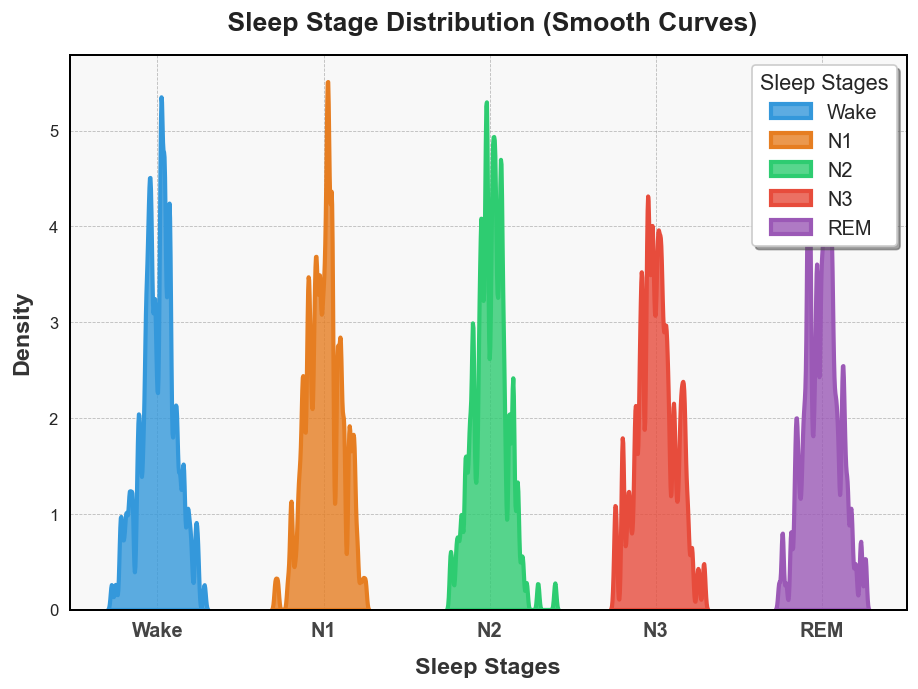
\includegraphics[width=0.9\linewidth]{figures/sample distribution plot pdf.png} % Replace with actual figure
        \vspace{5pt}
        {\textcolor{uwopurple}{\small Sampling Density Plot Showing Balanced Class Distribution}}

    \end{columns}

\end{frame}


\begin{frame}{Model Performance: Training vs Testing}

    \begin{columns}

        % Left Column: Accuracy Plot
        \column{0.50\textwidth}
        \centering
        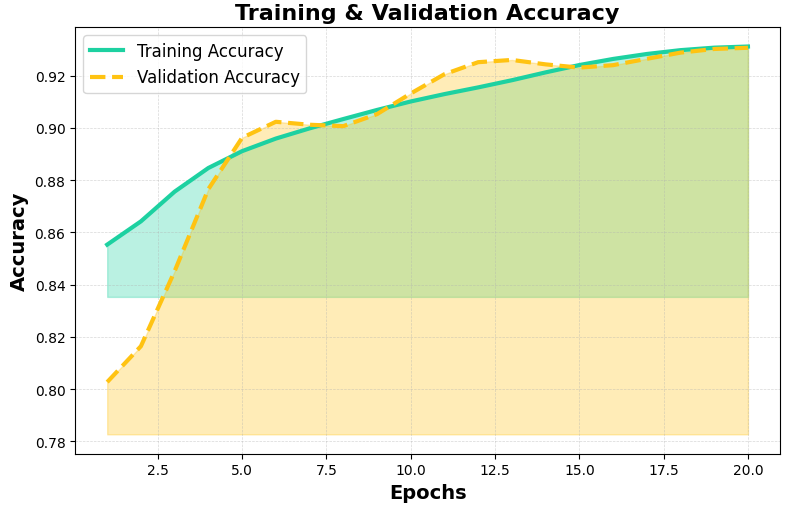
\includegraphics[width=1\linewidth]{figures/accuracy plot.png} % Replace with actual file
        \captionof{figure}{\textcolor{uwopurple}{ Accuracy Curve}}

        % Right Column: Loss Plot
        \column{0.50\textwidth}
        \centering
        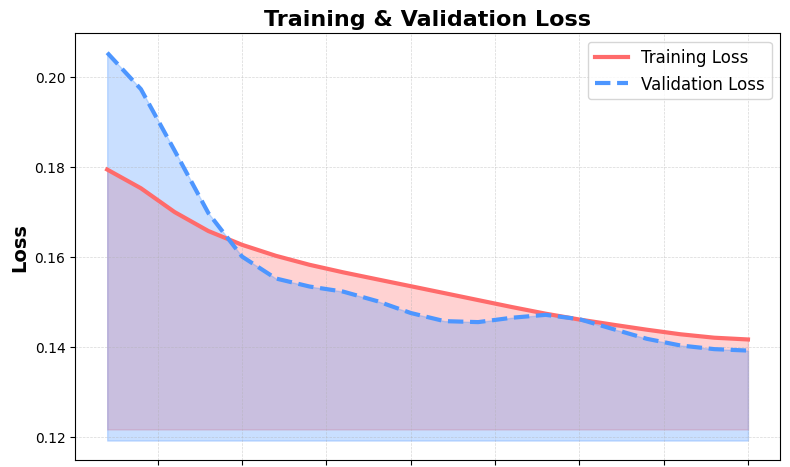
\includegraphics[width=1\linewidth]{figures/loss plot.png} % Replace with actual file
        \captionof{figure}{\textcolor{uwopurple}{ Loss Curve}}

    \end{columns}

\end{frame}



\begin{frame}{Model Evaluation: Confusion Matrix}

    \begin{columns}

        % Left Column: Precision, Recall, F1-Score Formulas
        \column{0.50\textwidth}
        \textbf{Performance Metrics}
        \vspace{10pt}
        
        \textbf{Precision:} 
        \[
        \text{Precision} = \frac{TP}{TP + FP}
        \]
        
        \textbf{Recall:} 
        \[
        \text{Recall} = \frac{TP}{TP + FN}
        \]

        \textbf{F1-Score:}
        \[
        \text{F1-Score} = \frac{2 \times \text{Precision} \times \text{Recall}}{\text{Precision} + \text{Recall}}
        \]

        \vspace{5pt}
        These metrics ensure a balanced evaluation of model performance across all classes.

        % Right Column: Confusion Matrix Plot
        \column{0.50\textwidth}
        \centering
        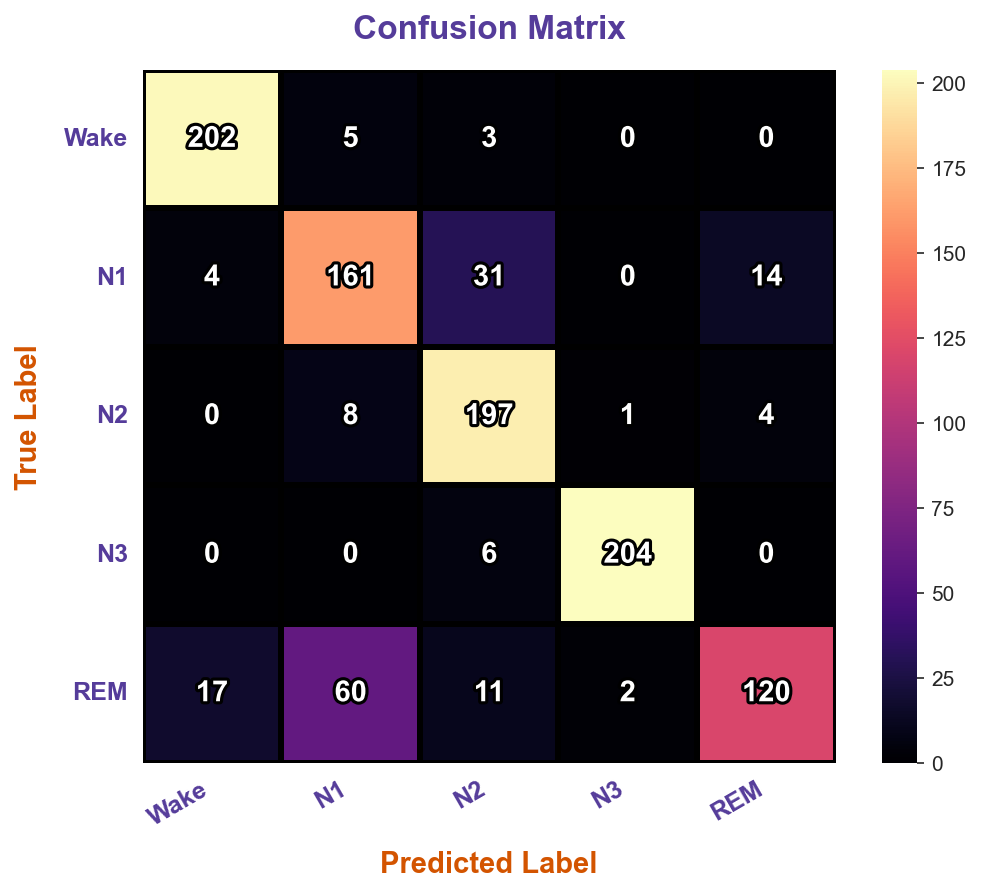
\includegraphics[width=0.9\linewidth]{figures/confusion matrix samples.png} % Replace with actual file
        \captionof{figure}{\textcolor{uwopurple}{Confusion Matrix }}

    \end{columns}

\end{frame}




\begin{frame}{Gradient Analysis: Training Progression}

    \begin{columns}

        % Left Column: Explanation of Training Behavior
        \column{0.50\textwidth}
        \textbf{Understanding Model Training Dynamics}
        \vspace{10pt}

      \begin{itemize}
            \item \textbf{Early Training (Epochs 0-5):} High loss, accuracy starts improving.
            \item \textbf{Mid Training (Epochs 5-15):} Loss steadily decreases, stable gradient flow.
            \item \textbf{Late Training (Epochs 15-20):} Accuracy plateaus, no severe overfitting.
        \end{itemize}

          \textbf{Conclusion:} The training process remains stable, with no vanishing or exploding gradients. 


        % Right Column: 3D Gradient Plot
        \column{0.50\textwidth}
        \centering
        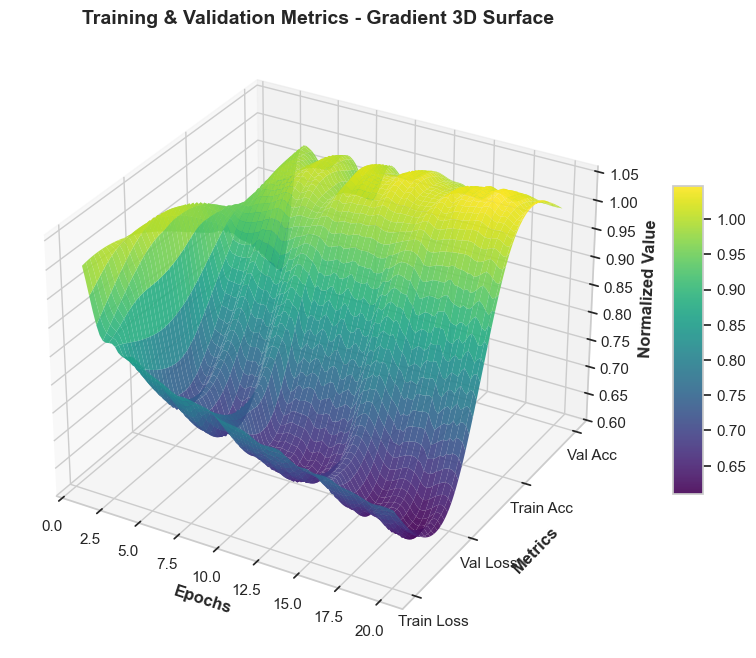
\includegraphics[width=0.9\linewidth]{figures/3d gradient.png} % Replace with actual file
        \captionof{figure}{\textcolor{purple}{Gradient 3D Surface: Training vs Validation Metrics}}

    \end{columns}

\end{frame}





\begin{frame}{Performance Metrics: Precision, Recall, F1-Score}

    \centering
    \textbf{Evaluating model performance across all classes using key metrics.}
    
    \vspace{10pt} % Add some space

    \begin{columns}
        % Left Column: Precision Bar Plot
        \column{0.33\textwidth}
        \centering
        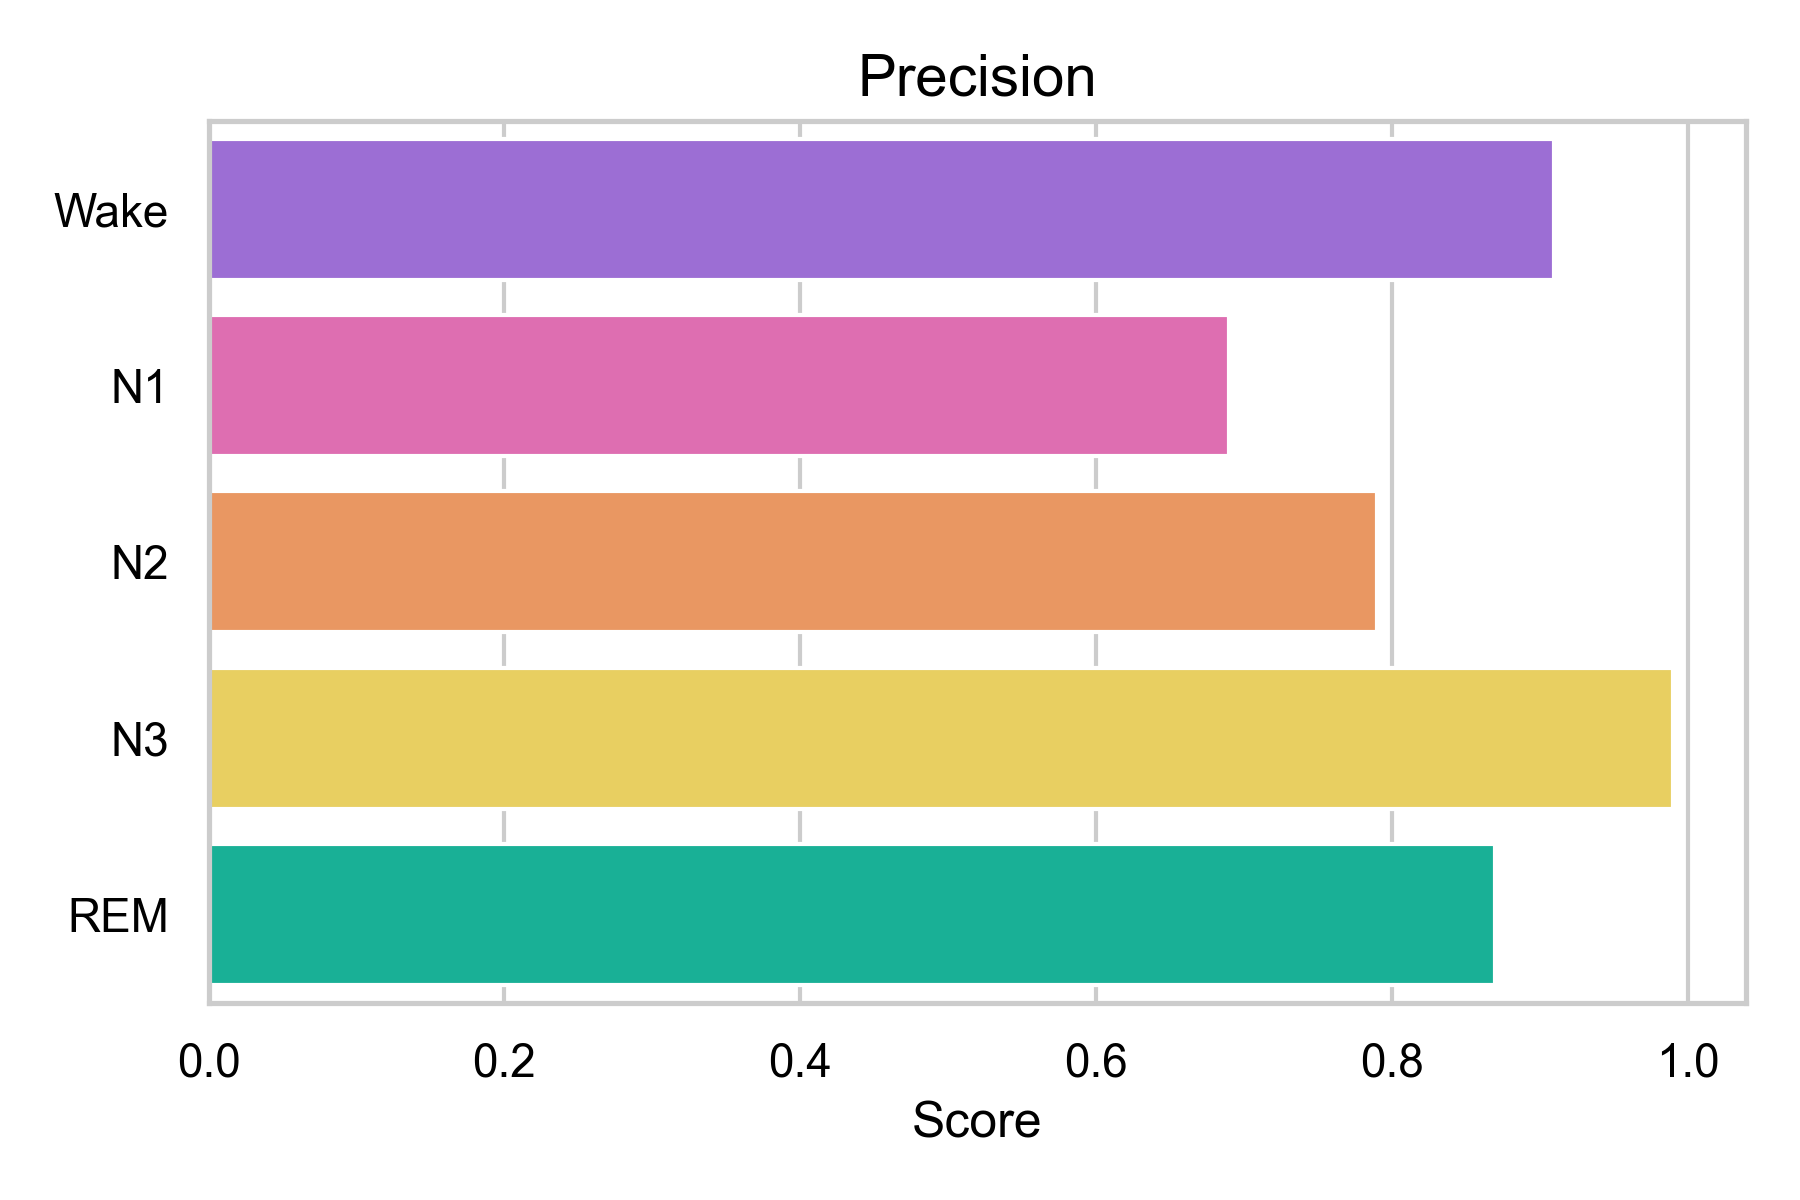
\includegraphics[width=\linewidth]{figures/precision_plot.png} % Replace with actual figure
        \captionof{figure}{\textcolor{purple}{Precision Scores per Class}}

        % Middle Column: Recall Bar Plot
        \column{0.33\textwidth}
        \centering
        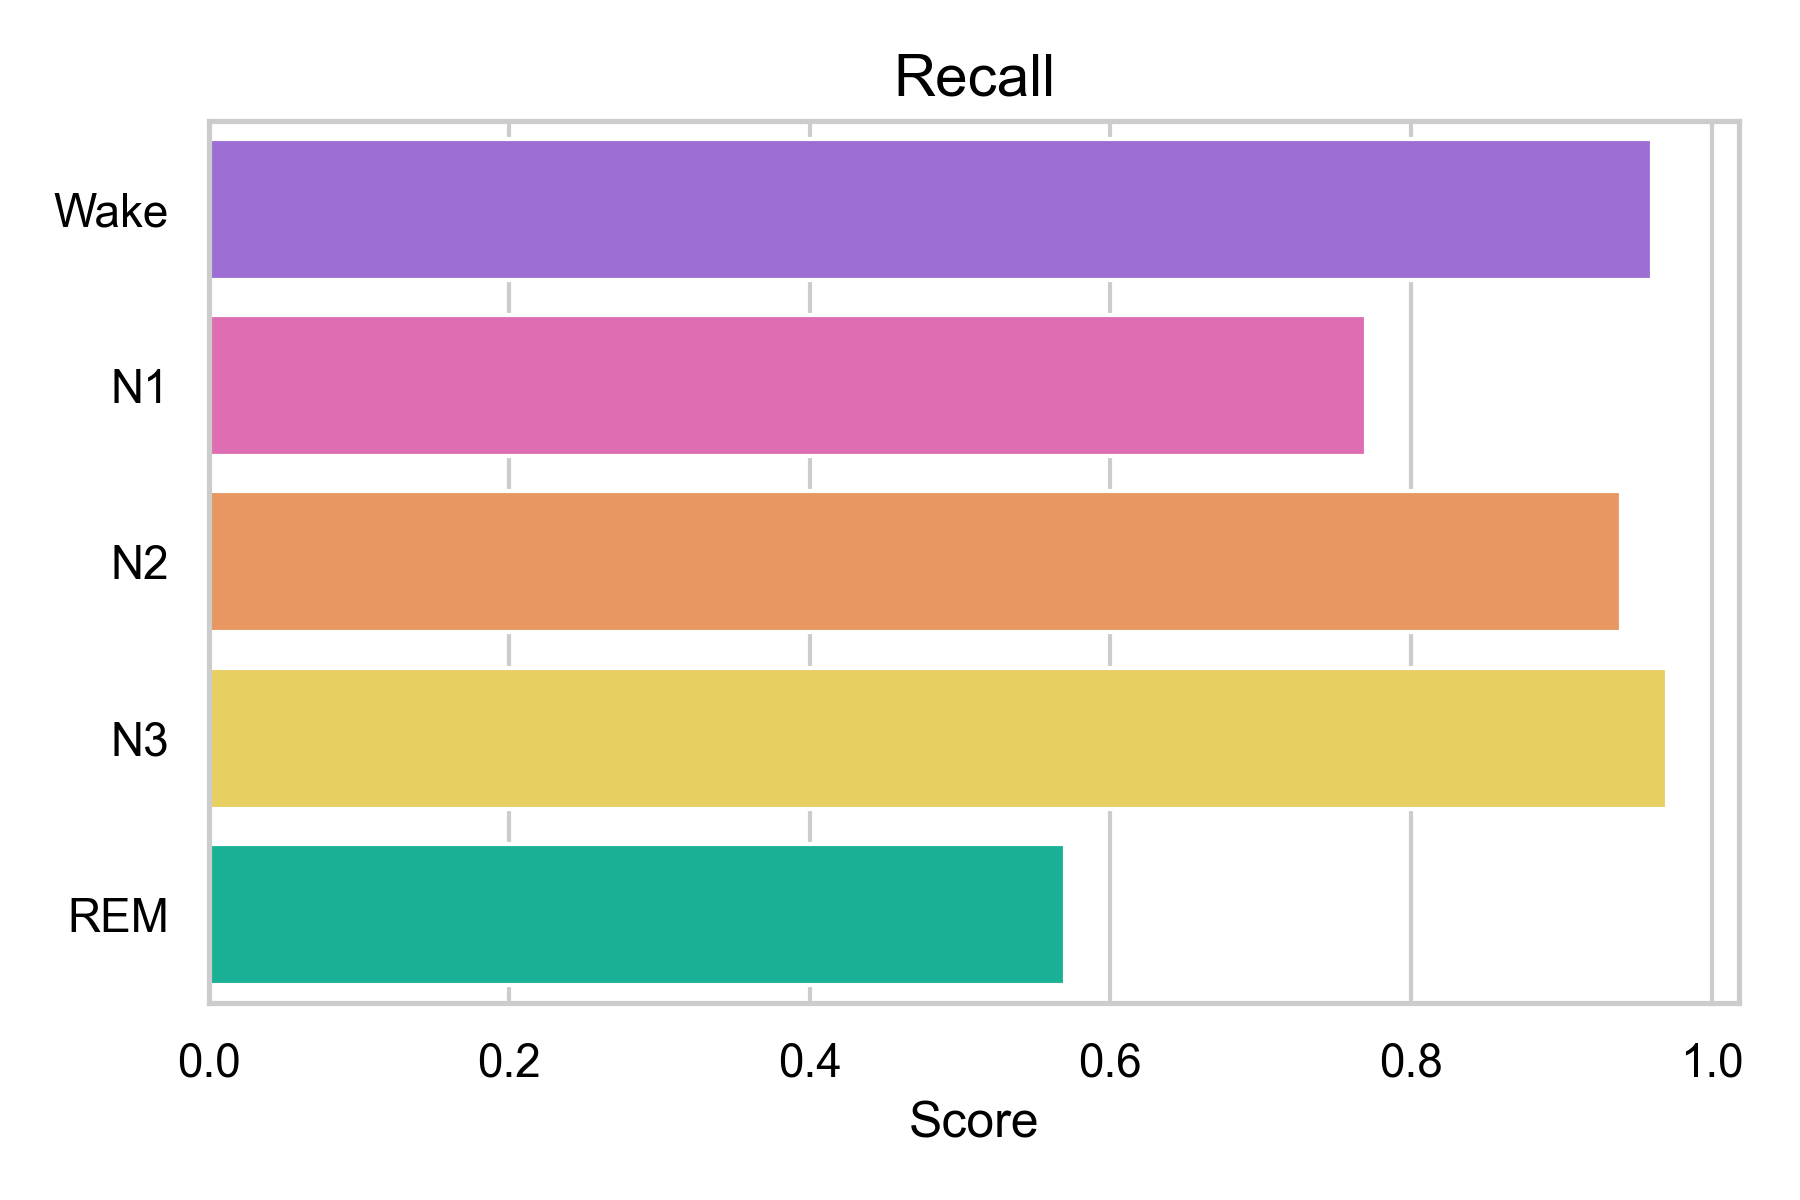
\includegraphics[width=\linewidth]{figures/recall_plot.png} % Replace with actual figure
        \captionof{figure}{\textcolor{purple}{Recall Scores per Class}}

        % Right Column: F1-Score Bar Plot
        \column{0.33\textwidth}
        \centering
        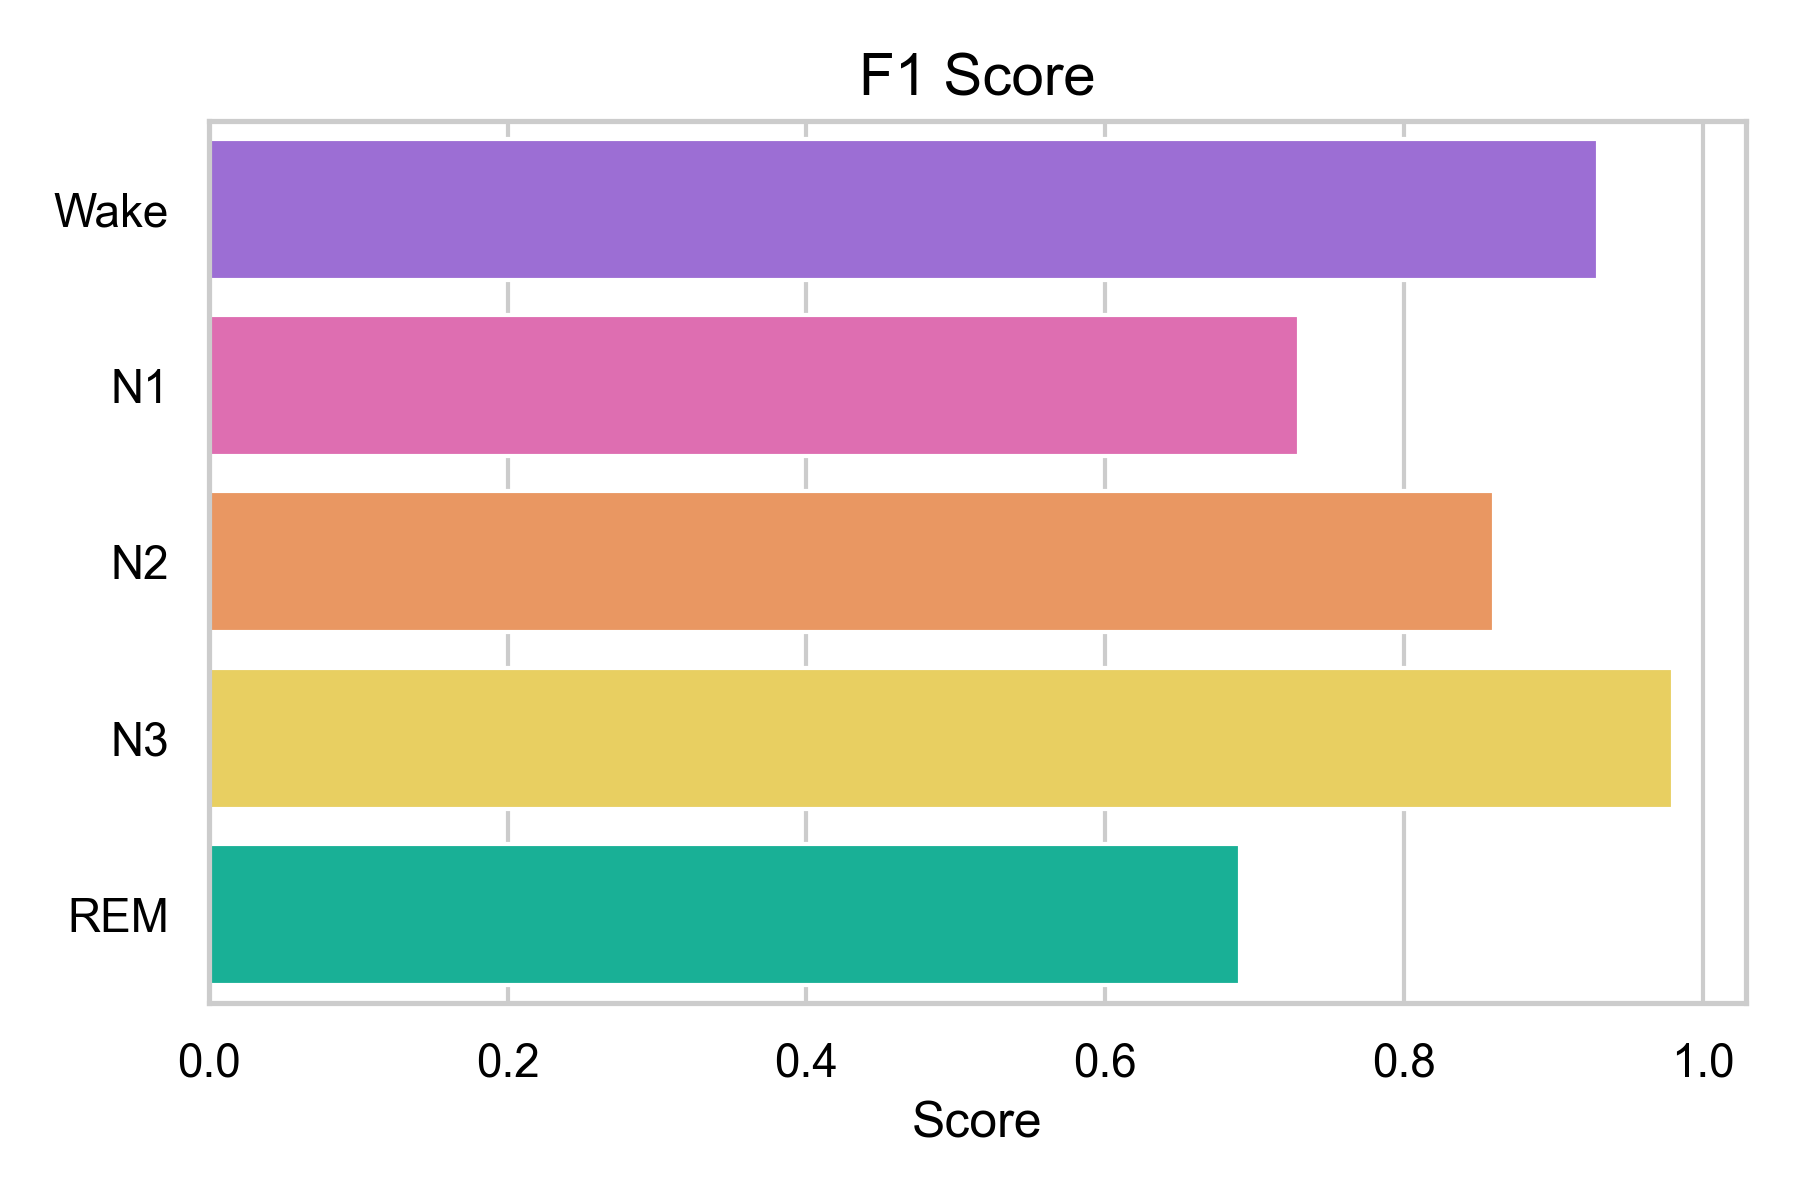
\includegraphics[width=\linewidth]{figures/f1_score_plot.png} % Replace with actual figure
        \captionof{figure}{\textcolor{purple}{F1 Scores per Class}}
    \end{columns}

\end{frame}

\begin{frame}{Feature Importance Analysis with LIME}

    \begin{columns}

        % Left Column: Explanation
        \column{0.5\textwidth}w
        \textbf{Understanding the contribution of different channels to model predictions.}

        \begin{itemize}
            \item We used \textbf{LIME} (Local Interpretable Model-agnostic Explanations) to analyze feature importance.
            \item The \textbf{EMG submental} and \textbf{EEG Pz-Oz} channels contribute the most to predictions.
            \item \textbf{EOG horizontal} has minimal importance, indicating lower relevance for classification.
            \item This insight helps optimize feature selection and improve model efficiency.
        \end{itemize}

        % Right Column: Figure
        \column{0.5\textwidth}
        \centering
        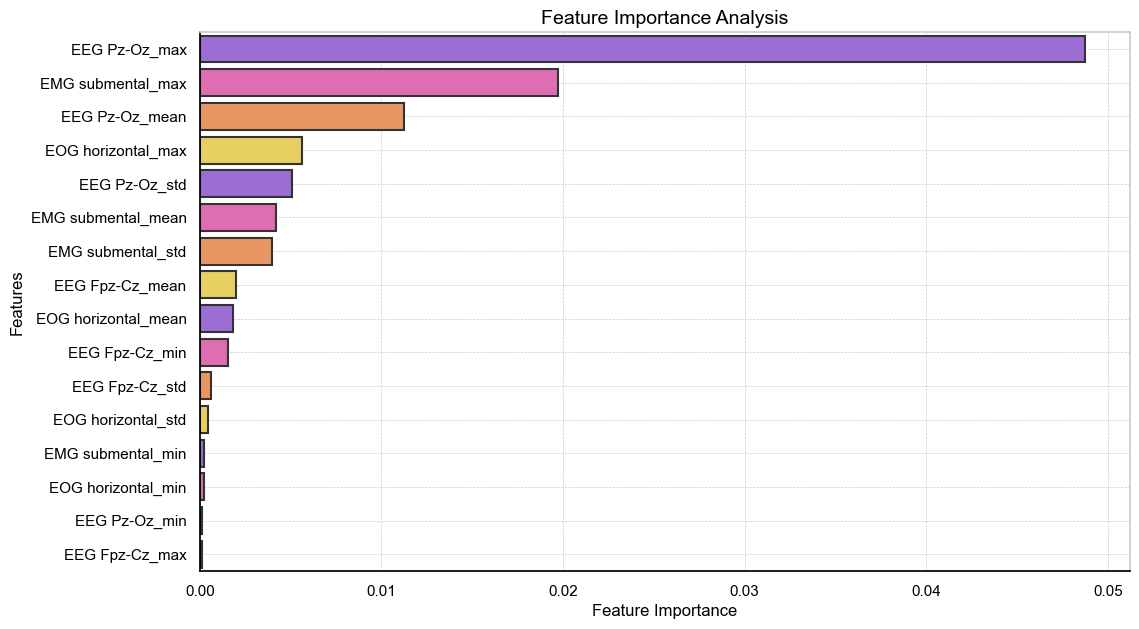
\includegraphics[width=0.9\linewidth]{figures/feature importance chanels analysis.png} % Replace with actual file path
        \captionof{figure}{\textcolor{purple}{Feature Importance Analysis for 4 Channels}}

    \end{columns}

\end{frame}




\begin{frame}{Future Plan: Enhancing Model Explainability}

    \textbf{Moving Towards Explainable AI for Sleep Staging}
    \vspace{0.5cm}
    
    \begin{itemize}
        \item \textbf{Why Explainability?}  
              - Medical experts need transparency in AI decisions for trust and adoption.  
              - Understanding how features influence sleep stage transitions is crucial.
              
        \item \textbf{Current Achievements:}  
              - \textcolor{blue}{\textbf{GCN:}} Captures spatial relationships between EEG channels.  
              - \textcolor{blue}{\textbf{Transformer:}} Captures temporal dependencies in sleep data.  
              - Achieved state-of-the-art accuracy using both approaches.
              
        \item \textbf{Next Steps:}  
              - Implement AI-driven methods to highlight critical sleep stage transition points.  
              - Develop feature attribution methods to understand the importance of each signal.  
              - Improve model interpretability to align with clinical expectations.
    \end{itemize}

\end{frame}



\begin{frame}{Future Plan: AI for Sleep Science and Clinical Use}

    \begin{columns}
        % Left Column: Explanation
        \column{0.55\textwidth}
        
        \textbf{Bridging AI and Healthcare}
        \begin{itemize}
            \item \textbf{Feature Importance:} Identify which EEG channels contribute most to predictions.
            \item \textbf{Clinical Relevance:} Provide insights that can be validated by sleep specialists.
            \item \textbf{Graph + Transformer Insights:}
            \begin{itemize}
                \item \textcolor{blue}{\textbf{GCN:}} Capturing inter-channel spatial dependencies.
                \item \textcolor{blue}{\textbf{Transformer:}} Learning sequential patterns across sleep cycles.
            \end{itemize}

                    \end{itemize}

        % Right Column: Block Diagram
       % Right Column: Block Diagram
\column{0.45\textwidth}
\centering
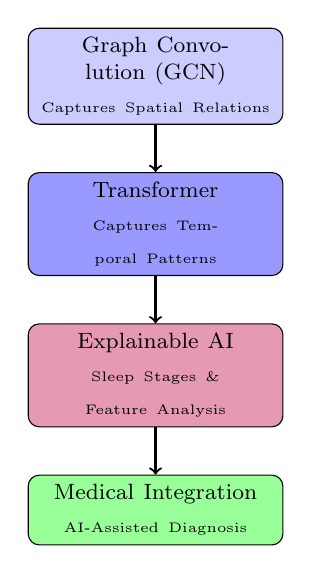
\begin{tikzpicture}
    % Nodes
    \node[draw, text width=3cm, align=center, fill=blue!20, rounded corners] 
        (gcn) {\footnotesize Graph Convolution (GCN) \\ \tiny Captures Spatial Relations};
        
    \node[draw, text width=3cm, align=center, fill=blue!40, rounded corners, below=0.6cm of gcn] 
        (transformer) {\footnotesize Transformer \\ \tiny Captures Temporal Patterns};
        
    \node[draw, text width=3cm, align=center, fill=purple!40, rounded corners, below=0.6cm of transformer] 
        (explainable) {\footnotesize Explainable AI \\ \tiny Sleep Stages \& Feature Analysis};
        
    \node[draw, text width=3cm, align=center, fill=green!40, rounded corners, below=0.6cm of explainable] 
        (medical) {\footnotesize Medical Integration \\ \tiny AI-Assisted Diagnosis};

    % Arrows
    \draw[->, thick] (gcn) -- (transformer);
    \draw[->, thick] (transformer) -- (explainable);
    \draw[->, thick] (explainable) -- (medical);
\end{tikzpicture}

    \end{columns}

\end{frame}


\begin{frame}{Conclusion}
    \begin{block}{}
    \justifying
    Our proposed SleepGCN-Transformer model achieves \textbf{93.12\% training accuracy} and \textbf{93.04\% validation accuracy}, demonstrating its effectiveness in sleep stage classification. The integration of \textbf{Graph Convolution Networks (GCN)} captures spatial dependencies across EEG, EOG, and EMG channels, while the \textbf{Transformer} extracts temporal patterns. The use of \textbf{Focal Loss} enhances class balancing, improving performance on underrepresented sleep stages. Feature importance analysis highlights \textbf{EMG and EEG Pz-Oz} as key predictors. This robust approach lays the foundation for future work in \textbf{Explainable AI}, enabling medical professionals to interpret AI-driven sleep diagnostics effectively.
    \end{block}
\end{frame}

\end{document}